% !TeX spellcheck = en_US
\documentclass[
	english,
	ruledheaders=section,%Ebene bis zu der die Überschriften mit Linien abgetrennt werden, vgl. DEMO-TUDaPub
	class=report,% Basisdokumentenklasse. Wählt die Korrespondierende KOMA-Script Klasse
	thesis={type=master},% Dokumententyp Thesis, für Dissertationen siehe die Demo-Datei DEMO-TUDaPhd
	accentcolor=9c,% Auswahl der Akzentfarbe
	custommargins=true,% Ränder werden mithilfe von typearea automatisch berechnet
	marginpar=false,% Kopfzeile und Fußzeile erstrecken sich nicht über die Randnotizspalte
	%BCOR=5mm,%Bindekorrektur, falls notwendig
	parskip=half-,%Absatzkennzeichnung durch Abstand vgl. KOMA-Script
	fontsize=11pt,%Basisschriftgröße laut Corporate Design ist mit 9pt häufig zu klein
%	logofile=example-image, %Falls die Logo Dateien nicht vorliegen
]{tudapub}


% Der folgende Block ist nur bei pdfTeX auf Versionen vor April 2018 notwendig
\usepackage{iftex}
\ifPDFTeX
	\usepackage[utf8]{inputenc}%kompatibilität mit TeX Versionen vor April 2018
\fi

%%%%%%%%%%%%%%%%%%%
%Sprachanpassung & Verbesserte Trennregeln
%%%%%%%%%%%%%%%%%%%
\usepackage[english, main=english]{babel}
\usepackage[autostyle]{csquotes}% Anführungszeichen vereinfacht

% Falls mit pdflatex kompiliert wird, wird microtype automatisch geladen, in diesem Fall muss diese Zeile entfernt werden, und falls weiter Optionen hinzugefügt werden sollen, muss dies über
% \PassOptionsToPackage{Optionen}{microtype}
% vor \documentclass hinzugefügt werden.
\usepackage{microtype}

%%%%%%%%%%%%%%%%%%%
%Literaturverzeichnis
%%%%%%%%%%%%%%%%%%%
\usepackage{biblatex}   % Literaturverzeichnis
\bibliography{CitaviV2}


%%%%%%%%%%%%%%%%%%%
%Paketvorschläge Tabellen
%%%%%%%%%%%%%%%%%%%
%\usepackage{array}     % Basispaket für Tabellenkonfiguration, wird von den folgenden automatisch geladen
\usepackage{tabularx}   % Tabellen, die sich automatisch der Breite anpassen
%\usepackage{longtable} % Mehrseitige Tabellen
%\usepackage{xltabular} % Mehrseitige Tabellen mit anpassbarer Breite
\usepackage{booktabs}   % Verbesserte Möglichkeiten für Tabellenlayout über horizontale Linien
\usepackage{makecell}
\usepackage{subcaption}
\usepackage{placeins}

%%%%%%%%%%%%%%%%%%%
%Paketvorschläge Mathematik
%%%%%%%%%%%%%%%%%%%
%\usepackage{mathtools} % erweiterte Fassung von amsmath
\usepackage{amssymb}   % erweiterter Zeichensatz
%\usepackage{siunitx}   % Einheiten

\usepackage{graphicx}
\graphicspath{ {../images/} }

\usepackage[percent]{overpic}
%\usepackage{mwe}
\usepackage{tikz}

%Formatierungen für Beispiele in diesem Dokument. Im Allgemeinen nicht notwendig!
\let\file\texttt
\let\code\texttt
\let\tbs\textbackslash
\let\pck\textsf
\let\cls\textsf

\usepackage{pifont}% Zapf-Dingbats Symbole
\newcommand*{\FeatureTrue}{\ding{52}}
\newcommand*{\FeatureFalse}{\ding{56}}

\begin{document}

\Metadata{
	title=TUDaThesis - Abschlussarbeiten im CD der TU Darmstadt,
	author=Linnea Widmayer
}

\title{TUDaThesis -- Abschlussarbeiten im CD der TU Darmstadt}
%\subtitle{Subtitle}
\author[L. Widmayer]{Linnea Widmayer}%optionales Argument ist die Signatur,
%\birthplace{Geburtsort}%Geburtsort, bei Dissertationen zwingend notwendig
\reviewer{Nico Faul \and Prof. Thomas Burg}%Gutachter

%Diese Felder werden untereinander auf der Titelseite platziert.
%\department ist eine notwendige Angabe, siehe auch dem Abschnitt `Abweichung von den Vorgaben für die Titelseite'
\department{etit} % Das Kürzel wird automatisch ersetzt und als Studienfach gewählt, siehe Liste der Kürzel im Dokument.
\institute{IMNS}
%\group{Arbeitsgruppe}

\submissiondate{\today}
\examdate{\today}

% Hinweis zur Lizenz:
% TUDa-CI verwendet momentan die Lizenz CC BY-NC-ND 2.0 DE als Voreinstellung.
% Die TU Darmstadt hat jedoch die Empfehlung von dieser auf die liberalere
% CC BY 4.0 geändert. Diese erlaubt eine Verwendung bearbeiteter Versionen und
% die kommerzielle Nutzung.
% TUDa-CI wird im nächsten größeren Release ebenfalls diese Anpassung vornehmen.
% Aus diesem Grund wird empfohlen die Lizenz manuell auszuwählen.
%\tuprints{urn=XXXXX,printid=XXXX,year=2022,license=cc-by-4.0}
% To see further information on the license option in English, remove the license= key and pay attention to the warning & help message.

%\dedication{Für alle, die \TeX{} nutzen.}
\maketitle

\affidavit% oder \affidavit[digital] falls eine rein digitale Abgabe vorgesehen ist.
% Es gibt mit Version 3.20 die Möglichkeit ein Bild als Signatur einzubinden.
% TUDa-CI kann nicht garantieren, dass dies zulässig ist oder eine eigenhändige Unterschrift ersetzt.
% Dies ist durch Studierende vor der Verwendung abzuklären.
% Die Verwendung funktioniert so:
%\affidavit[signature-image={\includegraphics[width=\width,height=1cm]{example-image}}, <hier können andere Optionen wie z.B. affidavit=digital zusätzlich stehen>]

\chapter*{Acknowledgment}

% !TeX spellcheck = en_US
First I want to thank Prof. Thomas Burg for his advice and support. My gratitude goes to Nico Faul for his guidance throughout my whole master thesis. Last I want to thank my family, partner and friends for motivation and support especially in the writing process of this thesis.

\chapter*{Abstract}

% !TeX spellcheck = en_US
Light microscopy and Electron microscopy are both widely used method to examine samples. Light microscopy makes observation possible over the visible light spectrum. In combination, fluorescence can be used to stain certain parts of a sample. In electron microscopy, structures to the smallest of scale is made visible by an electron beam. The distribution of different atoms is also observable. This complements both microscopy methods with each other.

As both microscopy methods are fundamentally different, sample preparation has different goals to enable each microscopy method. Most similar is the fixation of specimen with vitrificated ice is used in cryo light microscopy and cryo electron microscopy. In preparation, different sample holders are used. Generally, it is possible to combine cryo-light microscopy and cryo electron microscopy on the same sample with strong limitation. This results as sample holders optimized for one microscopy method are not designed for the other microscopy method.

In this master thesis, methods to switch sample holders are investigated. For this, two methods for separating ice layer including specimen from the sample holders are evaluated. A layer between sample holder and ice layer is designed. The layer is used to enable detachment of the ice layer to switch the sample slide between microscopy methods. 

The first idea is to dissolve a lipid layer between ice and sample holder for separation. A sacrificial layer containing lipids is designed. The sample holder is coated in parylene to decrease adhesion of ice on the sample holder. Solvents are tested regarding solubility at room- and cryogenic temperature. Results show that dissolving lipids is generally an endothermic process. This shows that dissolving the lipids DOPC and EGG-PC at cryogenic temperatures is too slow to dissolve a sacrificial layer. 

%TODO
The second idea is to mechanically detach the ice layer. To archieve this, a layer between sample and ice layer is used to reduce adhesion. A lipid and parylene layer as well as PDMS layer are examined. 

To be able to mechanically lift off the ice layer without destroying the specimen, all assemblies are cooled to \SI{-140}{\degreeCelsius}. A lifting assembly named "finger" uses the temperature dependent viscosity of Hydrofluorether to attach and detach to the ice layer. Baths filled with liquid nitrogen are used for sample preparation. A modified inverted fluorescence microscope is used to confirm successful detachment.

PDMS is tuned to reduce adhesion. The effect of plasma treatment is researched by tensile testing at room temperature on 1:2 base coat to curing agent ratio. The results show an increase of tensile strength of PDMS of up to 6 fold of untreated PDMS. On the other hand, this is not the case for mixture ratio with higher base coat content. The PDMS layer gets brittle and reduces adhesion in that way.

At cryogenic temperatures, sample holders coated with plasma treated PDMS and parylene/lipids are compared to each other. A successful detachment was archieved with a PDMS mixture ratio of 4:1. In future, assemblies should be improved and new ways of loosening the ice layer should be researched.



\tableofcontents

\chapter{Introduction}

	% !TeX spellcheck = en_US

Light microscopy (LM) is the simplest and most commonly used to magnify small objects and structures. There are many building varieties for different applications with different magnification ranges. In general, two building variation exist: Transmission LM do let light pass trough the sample to create an image. Reflective LM uses the reflecting light from the sample for imaging. 

For example, some light microscopes have additional fluorescence filters to detect fluorescence signals. These filters allow only the specific wave length emitted by a fluorescent molecule to pass. As a light source, filtered white light and lasers can be used, since only a specific wavelength range excites fluorescent molecules.

In LM many new advancements are still made. The Abbe criterium is the major limit for many light microscopes. However, multiple modified LM methods exist which are able to increase the resolution beyond this limit \cite{Heintzmann.2006}.

Electron microscopy (EM) is another imaging method being used: With electrons, resolutions down to the size of atoms are possible. The smallest structures in sub nanometer scale are observable with this method. Even the distribution of certain elements is detectable. Also the creation of 3D images are possible.

In EM, water containing structures must be fixated. One way to archive fixation of the specimen is to freeze the water to ice at cryogenic temperatures. With rapid cooling below \SI{-120}{\degreeCelsius} within tenths of milliseconds, vitrified ice which is amorphic and does not destroy structures by forming ice crystals is reached  \cite{Wowk.2010}. This requires low thermal conductivity which is only achievable with small and well thermal conducting sample holders. To hold the ice structure, all setups including microscopes to handle the specimen needs to be cooled below \SI{-120}{\degreeCelsius} to prevent subsequent crystallization of the ice.

To reach transparency of the electron beam for cryo scanning electron microscopy (cryo-TEM), the sample is required to have a maximum thickness of \SI{100}{\nano\meter} and containing only lighter elements. Additionally, a thin film in combination of a metal grid is used as a sample holder \cite{Danino.2012}. This grid does not deliver a regular background. Additionally, the sample needs to have low absorption of light in the visible spectrum in case a laser being used. If the contrast is too high, the sample is damaged trough light absorption and resulting heat.

For cryo-LM, the thin ice layer is frozen onto a thin sapphire disk. also here the thickness is limited by thermal conductivity to reach the vitrified state. The surface needs to be transparent in visible light or with low contrast \cite{Faoro.2018}.

Conveniently, the process of sample preparation for cryo-LM and cryo-EM is very similar. Still, the sample holder used for LM and EM are very limited inter operable. This grid does not deliver a regular background for reflective EM. Also a grid is not completely transparent for light for transmissive LM. also the grid absorbs visible light, limiting the use of lasers. The slides used in LM are mostly too thick for EM. Sometimes heavier elements are used too. Additionally some form of metal grid must be added for EM. 


Nevertheless, combining LM and EM on the same sample brings big advantages: The larger scale of LM and the use of multiple wavelengths combined with fluorescence and high resolution on the same sample does make studying samples easier. In this master thesis, a method for using cryo lLM and cryo-EM on the same sample is examined. To make this possible, the sample must be transferred to different sample holders between cryo-LM and cryo-EM without destroying the sample. To achieve this, a layer between ice and sample holder is engineered to enable detachment and transfer to another sample holder (Fig. \ref{fig:layersingeneral}).

\begin{figure}[hbt!]
	\centering
	\input{../images/Zeichnung_Layers_in_general.pdf_tex}
	\caption{Depiction of a sample. The specimen is frozen inside the ice layer. The sample holder and ice layer are connected by an additional engineered layer. In this master thesis, the additional layer is varied to allow separation of the ice including the specimen from the sample holder.}
	\label{fig:layersingeneral}
\end{figure}


\section{Task and requirements}

There are several requirements for this engineered layer: The layer must be thin to keep thermal conductivity high at freezing. The layer also must be hydrophilic and even to  enable freezing a regular thin ice layer on top. The engineered layer should not disturb LM or EM. 

The order of which kind of microscopy is performed first has an influence on the design of the layer. As the thickness and the design of the sample holder is less restrictive at LM, designing the layer for this environment is also easier. Therefore, LM is performed first in the final process. Then the ice layer is transferred to a grid. After this, cryo-EM is performed.

There are several challenges to perform a sample holder change: First, high wettability is needed when plunge-freezing. Wettability highly increases adhesion of ice on the rest of the sample. Second, the engineered layer is thin and covered by ice and sample holder. Therefore access to the layer is limited by solvents or other liquids. Third, the ice layer must stay in a vitrified state in the whole process. Last, many characteristics are temperature dependent. Results of experiments done at room temperature or close to freezing point are not easily transferable at \SI{-140}{\degreeCelsius}. For example, even mechanical stability and adhesion forces of all layers varies over temperature. Therefore everything needs to be validated at cryogenic temperatures \cite{Makkonen.2012}.

To fulfill all the requirements, following ideas are pursued. A sacrificial layer between sample holder and ice could be dissolved. The ice layer will float separately in the solution and could then be transferred to another sample holder. The second idea is to mechanically separate a piece or the hole ice layer from the sample holder. The layer must be designed in a way to reduce adhesion and posses high wettability at the same time. Also the forces applied must be strong enough for separation.

%First, I investigated lipids for positive characteristics for usage as a sacrificial layer. Second, different layers are tested for low ice adhesion. Also different parameters on the mechanical setup are tested.

\section{State-of-the-art}
\label{section:Stateoftheart}

Ice removal is needed in multiple commercial applications. Most strategies are only applicable in temperatures down to \SI{-30}{\degreeCelsius}. Since the ice layer in the demonstrated application needs to stay vitrificated at under \SI{-140}{\degreeCelsius} or even lower, only few anti-frosting methods are feasible. For example the active anti-frosting strategy of heating the ice is not possible, as the specimen must stay contained within the ice layer.

There are four passive anti-frosing strategies: Inhibition of ice nucleation is achieved by using surface inherent properties to prevent ice crystals from forming. Retardation of frosting removes water to prevent icing on the surface with water repellent properties such as the lotus effect. Mitigation of frost accumulation prevents already formed ice droplets from further accumulating and forming an ice layer. Last a reduction of ice adhesion on the surface prevents ice droplets to stay on the surface. Other forces like wind or gravity removes ice droplets and keeps the surface ice free \cite{Yang.2021}. 

Out of the four passive anti-frosting strategies, only one is applicable at cryogenic temperatures. The reduction of ice adhesion can be used to decrease the force needed to separate the ice layer mechanically. This can be done by using a hydrophobic surface with general low adhesion or with surface structuring. In contrast, Inhibition of ice nucleation, retardation of frosting and mitigation of accumulation only inhibit the freezing process itself and are therefore not applicable.

In industrial application, one commonly used coating to reduce adhesion of ice is Polydimethylsiloxane (PDMS). PDMS is a polymer which is widely used in different applications like in fabrication of micro channels, chip manufacturing, aerospace industry and medical tools. PDMS properties are for example its hydrophobility, biocompatability and electric insulating capabilities. Also PDMS is cost effective and allows rapid prototyping, molding and thin coatings \cite{Wolf.2018}. Additionally, PDMS is modifiable with additives.

One example in which the low ice adhesion potential of PDMS is illustrated is the passive deicing of Aircrafts in flight. As ice can influence the air flow around the wing an the body, which induces turbulence and reduces lift. Ice protection is therefore critical for a save and stable flying. In \cite{Liu.2018}, PDMS is tuned for optimal characteristics in flight. To test the surfaces, flight conditions of \SI{0.5}{\bar} and \SI{-12}{\degreeCelsius} are simulated. Fluorinated PDMS with and without silica nanoparticles are compared to aluminum, showing better resistance against ice growth. The different coatings are also examined regarding contact angle of water and surface roughness. Also the stability of the surface is relevant as ice formation and impacts can also wear down the coating itself. 

To create PDMS surfaces in labs Dowsil Sylgard 184 Silicone elastomer is widely used\cite{DOW.}. The PDMS kit includes a curing agent and base coat component. The specified mixture ratio is 10 base coat to 1 curing agent in weight (10:1). In some applications, other mixture ratios are used and additives are added for tuning PDMS.

For example, adhesion forces of ice on PDMS varies with different mixture ratios. In \cite{IbanezIbanez.2022}, PDMS is investigated in 3:1 to 1:50 weight ratio. The mixture is given into a mold and afterwards fully cured. An ice block is frozen on top of the PDMS. Using a pulling machine the maximum tensile and shear forces for detaching ice from PDMS are determined. Results show that mixture ratios 10:1 to 1:3 have significant lower adhesion forces on ice. At for example at 2:1, the shear mode is just under \SI{20}{\kilo\pascal} and the tensile mode around \SI{30}{\kilo\pascal}. 

Plasma curing is commonly used as PDMS treatment. Plasma treatment used for increasing wettability and adhesion. Plasma treatment is changing the chemistry of the polymer chains on the surface. Charged Oxygen Ions are deposited on the surface. these Ions make the surface temporarily hydrophile and increasing water adhesion. The Ions change the structure of the PDMS is permanently by oxidation. In some cases, cracks form as the surface oxidizes to a silica like form.

In \cite{Owen.1994}, the influence of different gasses on PDMS plasma treatment are examined. Oxygen, Nitrogen, Argon and Helium are compared on the effect on wettability, adhesion and cracking. Thin PDMS sheets are used with unknown composition. They found similar results between gasses. All gasses produced a thin and brittle surface with cracks and high wettability. Based on these results, used gas is not a significant factor for plasma activation. Therefore using only air (mainly a mixture of nitrogen and oxygen) is sufficient to determine the effect of plasma treatment.

In \cite{Ohishi.2017}, the influence of plasma treatment on Mixture ratios of 50:1 to 100:1 is described. A thin layer of those PDMS mixtures is put onto a preformed PDMS piece with lower mixture ratio. The preformed piece is used to apply shear stress to the surface by stretching the lower PDMS form piece. Therefore only tensile force are examined. It shows no significant difference between described mixture ratios. It also shows that higher plasma treatment leads to more brittle surfaces, reducing the force needed to break the PDMS Layer by $90\,\%$.

PDMS properties are also temperature dependent. In \cite{Zhang.2020}, multiple characteristics are determined for cryogenic temperatures. The PDMS is prepared with the standard mixture ratio of 10:1. The compressive strength increases with lower temperatures until \SI{-123.15}{\degreeCelsius}. At this temperature, the compressive strength reaches a maximum of \SI{224.50}{\mega\pascal} in average. At lower temperatures, the PDMS gets brittle. At \SI{-150.15}{\degreeCelsius} PDMS has a compressive strength of \SI{106.99}{\mega\pascal}.

%&The effect of Plasma activation between mixture ratios is mostly unknown. At mixture ratios above 50:1 base coat to curing agent, no significant differences between plasma activation is observed \cite{Ohishi.2017}. 



	
\chapter{Method}

	% !TeX spellcheck = en_US

(vielleicht absatz dass die Arbeit größtenteils aus praktischen Versuchen bestand???)

To find a working solution, many experiments are conducted. 

\section{Phospholipids}
\label{section:metodeLipide}

Phospholipids are the building block of membranes in nature. They are made of two long nonpolar carbon chains and a polar head. A membrane is a bilayer of Phospholipids with the hydrophobic carbon chains oriented inwards and the hydrophilic head pointing outwards. They are also natural detergents, as they can bind to hydrophobic waste forming an emulsion, making them removable with polar liquids like water \cite{SriramaM.BhairiPh.D..}.

Phospholipids are solvable in some common solvents. To apply Phospholipids, a slide is dipped into the solvent. When the solvent dries out, the lipids are binding to the surface of the slide, forming a layer with varying homogeneity. this layer can be removed with the same solvents. If the ice layer is frozen onto the lipid layer, the lipids can be solved at cryogenic temperatures, detaching the ice. But to solve this layer, a high solubility at cryogenic temperatures is required. 

% as the surface of the sacrifical layer is only on the edge of the sample.!

\subsection{Parylene}

Parylene is a hydrophobic polymer used as a coating to repel particles, including water and ice. Parylene is also biocompatible and used in medicine and biology (QUELLE?).

Parylene is not usable without a second layer on top. Parylene hydrophobicity does not allow water to spread during plunge freezing. with plasma activation, the surface is now hyrdophilic, but ice adheres to the parylene too strong to mechanically detach. also parylene cannot be solved with a solvent as a sacrificial layer.

For this reason, lipids are used in combination with parylene (Fig. \ref{fig:sacrificial layer}). The hydrophobic chains of the lipids adhere to the parylene. The polar head allow water to spread evenly over the surface. Solving the lipids with a solvent will detach the ice layer from the slide. Parylene additionally prevents (re-) attachment through holes in the lipid layer. 

\begin{figure}[hbt!]
	\centering
	\input{../images/Zeichnung_Layer_Lipide_parylene.pdf_tex}
	\caption{Layers of a Sample. The Lipid layer is used as a sacrificial layer. To reach the layer with a solvent, the only contact surface is to the edge. To get a fast and reliable process, a solvent with high solubility is needed.}
	\label{fig:sacrificial layer}
\end{figure}


\subsection{Preparation of lipid coated slides}

To create the slides with parylene and lipids, a cover glass (\SI{5}{\milli\meter} diameter) is used as base. the cover glass is coated with a thin layer of parylene. The coated cover glass is dipped into lipid solution. The cover glass is dried, leaving behind a lipid layer. The prepared slides are then used in plunge freezing.

Two different kind of lipids are used: DOPC and EGG-PC. DOPC is storaged as a powder. The DOPC powder is solved in Ethanol ($25\,\si{\milli\gram}/1\,\si{\milli\liter}$ lipid to solvent) for application. 
EGG-PC is shipped solved in chloroform in two different ratios: $25\,\si{\milli\gram}/1\,\si{\milli\liter}$ and $10\,\si{\milli\gram}/1\,\si{\milli\liter}$. The solution is shipped in phioles.

The lipid solution is transferred into several small bottles. small bottles are chosen because solution forms a lubrication film on the thread of the lid. this prevents the lid from closing airtight. This leads to evaporation of the solvent over time, making the bottle unusable. In the coating process, solution often drops onto the threads, making a bottle only usable in one coating session. By splitting the solution into multiple flask, more slides can be covered from one batch of solution.

\subsection{solubility lipids}

These tests are conducted to find a fluid to solve a sacrificial layer out of lipids. (BEDINGUNGEN SACRIFICIAL LAYER? ODER KAM DAS SCHON?)

Two consecutive solubility experiments are proposed. The first experiment is conducted at room temperature. the aim is to find solvents with high solubility at room temperature. the candidates with high solubility are then tested in the next experiment at cryogenic temperature. the aim is now to find solvents with also high solubility at cryogenic temperatures. The first experiment is conducted as there are only three baths available at cryogenic temperature. therefore the throughput for experiments is limited.

\subsubsection{at room temperature}

The Solvent are chosen based on availability, freezing point and safety. The solvents are all readily available in the laboratory. Some were ordered before the test. Also all chosen solvent are save to use in a well ventilated room. The followup experiment cannot be conducted under a extractor hood as too much space is taken up with the experiment. Also the solvent or solvent mixture needs to stay liquid at around \SI{-140}{\degreeCelsius} to assure that the ice layer on top stays vitrified. The tested substances are 4-Methyl Pentene, 3-Methyl Pentene, 1-Pentene, Isopentane, 1-Propanol, Pentane and Ethanol. 

Each solvent is put in a separate bottle. The lipid coated slides are prepared as previously described. For each solvent, a slide is put in the corresponding bottle. After \SI{15}{\minute}, the slides are removed and examined. The results are documented in a list. When all streaks caused by the lipid layer disappeared, the solvent is tested in the next experiment.

\subsubsection{at cryogenic temperature}
\label{chapter:meltingtemp}


Solubility is temperature dependent. Most solutions are endothermic. this means energy is needed to solve another substance. Also the saturation point of the solution can change. Therefore, solubility needs to be tested at the same temperature as in application

The experiment is conducted at \SI{-140}{\degreeCelsius}. The solvents are given in liquid nitrogen cooled baths, which are regulated to the desired temperature. A slide is given into the cold solvent for \SI{15}{\minute}. Then the slide is examined for leftover streaks as before.

The freezing point of tested solvents are not all below \SI{140}{\degreeCelsius}] (Table \ref{table:SchmelztemperaturLösungsmittel}). Still, solvents with a high freezing point can be mixed with other solvents with lower freezing point to lower the freezing point of the mixture. Alternatively, the temperature can be raised over the freezing point, but this could risk the ice to loose the vitrified state.

\begin{table}[hbt!]
	\centering
	\begin{tabular}{|l|c|}
		\hline
		solvent & melting point in °C \\
		\hline
		\hline
		4-Methyl Pentene & -154 \\ 
		\hline
		3-Methyl Pentene & -154 \\
		\hline
		1-Pentene & -165 \\
		\hline
		Isopentane & -160 \\
		\hline
		1-Propanol & -126 \\
		\hline
		Pentane & -129 \\
		\hline
		Ethanol & -114 \\
		\hline
	\end{tabular}
	\caption{Melting Point in °C for tested solvents.}
	\label{table:SchmelztemperaturLösungsmittel}
\end{table}

In the end, experiments has proven that solving lipids fast and reliable is not possible with tested solvents. As all solvent lipid combinations are endothermic. finding a working solvent lipid combination is very unlikely, as almost all combination of solvent and lipids will be endothermic.

Additionally, some solvents tested are soluble in water. It is unknown whether the solvents could be solved or diffuse inside the ice layer at \SI{-140}{\degreeCelsius}. Therefore the ice layer could be changed in some undesired manner. if a sufficient solvent is found and the solvent is soluble in water, a potential change of the vitrified ice needs to be addressed.

\section{Detaching ice mechanically}

The next explored method is detaching the ice layer mechanically. For this, a lifting assembly is used. To make this possible, the bottom layer is engineered to reduce the adhesion of the ice. Also, as the assembly was not used in similar work before, different variables are addressed and examined.  

\subsection{Assemblies used at cryogenic temperatures}

The assembly used to lift up samples is called the "finger". The finger is made of two main parts. The first part is metal rod with a slightly pointed tip (Fig. \ref{fig:querschnittfinger}). The rod is cooled with cold nitrogen gas. Near the tip, the rod is temperature controlled with a temperature sensor and a heater. The second main part is a 3D printed part, containing the outer shell and routing of the cold gaseous nitrogen. The nitrogen is  directed downwards around the metal bar in an inner mantle for cooling. then, the Gas is directed upwards flowing through an outer mantle for additional cooling. Then the gas is exits through the output.

The Gas is supplied by a liquid nitrogen tank. Heaters are placed inside the tank to evaporate the liquid nitrogen. The volume is rapidly expanding at eveporation, resulting in fast gas flow. the cold nitrogen gas is routed by \SI{6}{\milli\meter} pneumatic tubing. at the inlet and outlet of the finger, festo connectors are fixed to allow easy maintenance. the inlet of the finger is connected to the liquid nitrogen tank. the outlet tubing exhausts the cold nitrogen into the atmosphere.

The finger is  mounted on three stages. additionally the stages are mounted on a track. the three stages allow fine adjustment of the finger position in X,Y and Z axis. Also, when the finger is attached to a surface, force can be applied by moving the stages in either direction. The Finger can also be moved along the track. In use, the assembly is clamped down on the track to prevent movement. when not in use, the assembly can be moved on the track to allow easy access of the area below the "finger".

\begin{figure}[hbt!]
	\centering
	\input{../images/ZeichnungFinger.pdf_tex}
	\caption{A cross-section of the "finger" assembly. The metal rod is cooled with cold nitrogen gas. the gas is routed from the inlet around the metal bar onto an outer layer to the outlet. The metal rod is temperature controlled by a temperature sensor and a heater. With HFE 7200 is applied to the tip, the finger can attach to a surface at cryogenic temperatures and apply force. }
	\label{fig:querschnittfinger}
\end{figure}

\begin{comment}
	\begin{figure}[hbt!]
		\centering
		\begin{overpic}[height=7cm]{TempFinger}%
			%\color{red}%
			%\put(49,48){\vector(0,-1){10}}%
			%\put(49,48){\makebox(0,0)[cb]{Mitte}}%
			%Beschriftung:
			\thicklines
			\put(42,15){\vector(-1,0){10}}
			\put(42,15){\makebox(0,0)[lb]{ Heater,}}
			\put(42,15){\makebox(0,0)[lt]{ Temperature sensor}}
			\put(3,50){\vector(1,0){20}}
			\put(3,50){\makebox(0,0)[r]{Steel Rod }}
			\put(5,96){\vector(1,-1){10}}
			\put(5,96){\makebox(0,0)[r]{Gas inlet }}
			\put(48,96){\vector(-1,-1){10}}
			\put(48,96){\makebox(0,0)[l]{ Gas outlet}}
			\put(17,0){\vector(2,1){10}}
			\put(17,0){\makebox(0,0)[r]{Tip }}
			% Gas Flow:
			%\put(21,45){\vector(0,-1){12}}
			%\put(19,33){\oval(4,4)[b]}
			%\put(17,33){\line(0,1){12}}
		\end{overpic}
		\caption{Querschnitt finger}
		\label{fig:querschnittfinger}
	\end{figure}
\end{comment}


On the tip of the finger, Hydrofluorether (here HFE 7200) is applied. HFE is an oil typically used as an cryoimmersion fluid \cite{Faoro.2018b}QUELLE ÜBERPRÜFEN!. Besides that, it has temperature dependent abilities. At freezing temperatures, it does not freeze into a solid at once. It gets more and more viscious before it freezes completely. this temperature dependency is used to first apply the HFE at higher temperatures with low viscosity and pull on the sample at low temperatures.

In the beginning a smaller bath is used (Fig. \ref{fig:KleinesBad}). The Small bath contains an elevated floor as work surface. embedded in the work surface are indents which are used as container holder. those container allow transport and long term storage of samples. Three elevated baths are installed above the work station. They are used for temperature controlling and containing other Liquids or tools. Also a Haven for a shuttle system is installed. The small baths and the haven are elevated over the second floor with an insulating layer, so a temperatures over \SI{-195.8}{\degreeCelsius} can be regulated. The liquid nitrogen is filled over the work surface, but not over the insulating layers to allow temperature controlling. The whole bath is insulated by Nitrogen gas flowing inside the 3D-printed shell of the bath. Then the Nitrogen gas is expelled from the brim, pointing from the outer edge radially to the rotation axis. In that way, the nitrogen gas separates the damp air in the room with the dry nitrogen gas inside the bath. Therefore ice formation inside the bath is inhibited.

This small bath and later the big bath are also used in combination with the "finger". The "finger" is positioned over the shuttle docked in the haven. The sample is fixed in the shuttle. with the stage, the position of the "finger" is manipulated. The Nitrogen gas also keeps the "finger" tip ice free.

The usage of the small bath in combination of the finger has its limitations: first, the space is small. The "finger" can be moved along the track, but the space still limits work freedom with pincers. Additionally, the smaller baths are not needed when using the finger. also the Shuttle needs to be tilted in a specific angle so docking and undocking of shuttle in the haven is possible. The work flow also allows only one shuttle at once, limiting throughput. Also Liquid nitrogen needs to be refilled often as the bath can only hold a small volume.

\begin{figure}[hbt!]
	\centering
	\begin{overpic}[width=10cm]{SmallBath}
		\white
		\put(40,25){\vector(1,1){10}}
		\put(40,25){\makebox(0,0)[r]{shuttle haven}}
		\put(20,45){\vector(1,0){15}}
		\put(20,45){\makebox(0,0)[r]{tool bath}}
		\put(73,35){\vector(-1,1){10}}
		\put(73,35){\makebox(0,0)[l]{ethanol bath}}
		\put(73,27){\vector(-1,1){10}}
		\put(73,27){\makebox(0,0)[l]{HFE bath}}
		%\put(49,76){\vector(-0.15,-1){3.4}}
		%\put(51,76){\vector(0.15,-1){3.4}}
		\put(48,65){\vector(-0.25,-1){2.8}}
		\put(52,65){\vector(0.25,-1){2.8}}
		\put(50,65){\makebox(0,0)[b]{container holder}}
		%\put(75,78){\vector(-2,-1){10}}
		%\put(76,78){\vector(-1,-2){4.5}}
		\put(75,72){\vector(-1,0){10}}
		\put(79,68){\vector(-1,-1){3.5}}
		\put(75,72){\makebox(0,0)[lt]{gas outlets}}
		\put(75,72){\makebox(0,0)[lb]{nitrogen}}
		\put(30,62){\vector(1,-1){10}}
		\put(30,62){\makebox(0,0)[rb]{work surface}}

		
	\end{overpic}
	\caption{Small Bath.}
	\label{fig:KleinesBad}
\end{figure}

During this master thesis, a second bigger bath is build (Fig. \ref{fig:GroßesBadMitFinger}). In general, the structure is similar. It also has an elevated floor as a work surface. The work surface is fabricated out of two plates screwed together. Indents are formed by holes in the upper plate. No baths are installed, but the space is planned in for later addition. The work surface is held in place by 3D printed holders which are fixed to the brim of the metal bath. Also two harbors can be mounted for parallel work on two separate shuttles. The harbors are screwed on an aluminum block. the aluminum block is temperature regulated. between the aluminum block and the work surface, a 3D-printed insulating layer is placed. Also both harbors can be mounted either flat or in an angle, depending of the 3D printed layer. The Bath is insulated with styrofoam and a rim with holes for warm nitrogen gas is placed on top. The holes are places along the inside of the longer perimeter, so the stream covers the whole area with minimal turbulence. This also keeps the inside ice free.

\begin{figure}[hbt!]
	\centering
	\begin{overpic}[width=10cm]{BigBathWithFinger}
		\white
		\put(24, 35){\vector(1,1){10}}
		\put(24, 35){\makebox(0,0)[t]{shuttle haven}}
		\put(46, 31){\vector(-1,1){10}}
		\put(46, 31){\makebox(0,0)[t]{temp. controlled aluminum block}}
		\put(25, 75){\vector(1,0){10}}
		\put(25, 75){\makebox(0,0)[r]{"finger"}}
		\put(15, 19){\vector(-1,-1){10}}
		\put(15, 19){\makebox(0,0)[l]{inlet warm nitrogen gas}}
		\put(50, 15){\vector(0,1){5}}
		\put(50, 15){\makebox(0,0)[t]{hole for refilling}}
		\put(40, 85){\vector(-1,1){5}}
		\put(40, 85){\makebox(0,0)[l]{cold nitrogen tubing}}
		\put(15, 58){\vector(0,-1){15}}
		\put(16, 58){\vector(0,-1){10}}
		\put(16, 58){\makebox(0,0)[b]{gas outlets nitrogen}}
		\put(32, 52){\vector(0,1){5}}
		\put(32, 52){\makebox(0,0)[t]{container holder}}
		\put(17, 88){\vector(0,-1){5}}
		\put(17, 88){\makebox(0,0)[b]{connection "finger" to stage}}
	\end{overpic}
	\caption{Big Bath with Finger.}
	\label{fig:GroßesBadMitFinger}
\end{figure}

To take pictures of the sample, an inverted microscope is rebuilt for cryo microscopy (Fig. \ref{fig:Mikroskop}). A box with a metal core is fixed to the bottom of the stage. an outer frame an the top of the box is temperature controlled. The box is supplied with cold nitrogen gas to cool the iron core. a haven is fixed to the iron core and placed over the objective. The haven is temperature controlled to \SI{-140}{\degreeCelsius} to make remains of HFE liquid and distinguishable. to keep the light path between haven and objective clear from ice and fog, a component reffered to as "glasses" is used(HIER REFERENZ ZUR ZEICHNUNG VON DER BRILLE?). It contains two parallel glass slides. Warm nitrogen gas is routed beween the glass slides and the lower glass slide and objective. Additionally, a filter is used for examining fluorescent samples.

The Shuttles are also used in cryo light microscopes. The Microscope used for cryotemperatures have an additional box installed, routing Cold nitrogen gas underneath a harbor, where the sample is placed. Heaters are placed around the box and under the harbor to archieve a constant temperature. On top of the Harbor, warm Nitrogen is blown so no ice is forming inside the optical path.

\begin{figure}[hbt!]
	\centering
	\begin{overpic}[width=10cm]{Microscope}
		\put(24, 45){\vector(1,0){10}}
		\put(24, 45){\makebox(0,0)[r]{cooled box}}
		\put(15, 50){\vector(1,0){10}}
		\put(15, 50){\makebox(0,0)[r]{frame}}
		\put(35, 25){\vector(1,0){5}}
		\put(35, 25){\makebox(0,0)[r]{objective}}
		\white
		\put(52, 33){\vector(-1,0){10}}
		\put(52, 33){\makebox(0,0)[l]{"glasses"}}
		\put(55, 52){\makebox(0,0)[c]{cold nitrogen gas supply}}
		\put(50, 75){\makebox(0,0)[b]{stage}}
		\put(59, 40){\vector(-1,0){10}}
		\put(59, 40){\makebox(0,0)[l]{gas outlet}}
		\put(32, 35){\vector(1,0){10}}
		\put(32, 35){\makebox(0,0)[r]{access shuttle}}
		
		
	\end{overpic}
	\caption{Modified microscope for cryo microscopy.}
	\label{fig:Mikroskop}
\end{figure}

The shuttle allows easy transportation of the sample without limiting the access to the sample. The sample is clamped down by a brace, which is also reffered to as "window". The "window" is fixed with two screws to the shuttle, holding the sample in place. the "window" gives access to the top side of the sample with a center hole for microscopy and "finger". A long rod with a thread at one side and a temperature insulated knob on the other side is used to screw into the sample. This allows easy transport between bath and microscope. 

\begin{figure}[hbt!]
	\centering
	\input{../images/Zeichnung_shuttle.pdf_tex}
	\caption{Shuttle for transporting a sample between bath and microscope. The "window" is clamped down by screws to the copper shuttle, holding the sample in place. Through the hole in the window, microscopy is done on the sample. The "finger" fit also through the "window" for pulling. For transport, a rod is screwed into the copper shuttle.}
	\label{fig:shuttle}
\end{figure}

On the other hand, small container with space for three $\varnothing$\SI{5}{\milli\meter} samples are used (Fig. \ref{fig:transportbox}). These are 3D Printed, modified version of other containers. a cap which is identical with the other versions of container is screwed on top with a special pencil. Inside the bath, the container fit into the indent. the cap is screwed next to the container, holding it into place. Also the container can be stored in the same container of the other version. This allows long term storage of samples with \SI{5}{\milli\meter} diameter.


\begin{figure}[hbt!]
	\centering
	\input{../images/Zeichnung_transportbox.pdf_tex}
	\caption{Small transport box for three samples. a cap is screwed onto the central thread. (WAS ZUM DECKEL SCHREIBEN). These boxes fit into storage units for long time storage.}
	\label{fig:transportbox}
\end{figure}

\FloatBarrier

\subsection{Process}

The goal is to mechanically lift a piece or the whole ice layer from the slide it is frozen to. In the whole process, the ice stays in the vitrified state. The sample is prepared in the bath. The "finger" is used to attach and pull on the ice layer with HFE. Also the microscope is used to take pictures of the sample without heating up the sample.

To try out the detachment with the "finger" in a repeatable manner, a core process is established for orientation. The sample is prepared and put in the bath. The copper shuttle part is placed in the harbor. With HFE, the sample is placed in the middle of the shuttle. The HFE helps the sample to stay in place before fixation. The window brace is placed on top and screwed down. The now prepared shuttle is transported quickly to the microscope. When the transfer is not possible within seconds, the shuttle is placed in a portable container with liquid nitrogen. After microscopy, the sample is placed into the bath unter the cooled finger. 

First, if not already done, cool down the "finger" to \SI{-140}{\degreeCelsius}. HFE is applied to the tip. The "finger" is lowered onto the sample while correcting the position with the stages until the HFE contacts and spreads over the sample. The temperature is reduced to \SI{-160}{\degreeCelsius} and waited until the sample and finger is cooled down. When the temperature is reached the finger is pulled up by turning the stage until detachment. Then the shuttle is transported to the microscope and the sample is analyzed. 

When detachment is successful, the ice piece hanging on the "finger" is placed on another shuttle. This is done by lowering the finger onto the new shuttle and raising the Temperature to \SI{-140}{\degreeCelsius}.

To collect first insight, samples with parylene and lipids (as described in Section \ref{section:metodeLipide}) are used first. different variables are determined which could significantly influence successful detaching. Then the different variables are examined with experiments to improve the reliability of the "finger". The different variables found in this thesis are discussed in the following sections.

\subsection{determining needed amount of glue}

Using the correct amount of HFE as glue is important for a high repeatability. Too little glue is not able to connect the finger to the sample. too much glue results into a thicker layer, which is the weakest link between finger and sample. additionally, the glue can spread underneath the "window" which is holding down the sample onto the shuttle. 

In first experiments, the HFE used as glue was applied with a pincer. TO archieve this, the HFE is given in a cold bath at -140°C. This stops HFE from evaporating. The thickened hfe is now scooped with pincers on the tip of the finger. Though the correct amount is only determinable qualitative.

As an effort to determine the correct amount of HFE a pipette is used. The HFE is pipetted at room temperature, because at lower temperatures the viscosity is already too high. While applying the HFE onto the desired surface, around $4\,\mu l$ is already evaporating. Also, sometimes the hfe does not land on the tip but on the side of the tip, where it is not very useful. 

In the first experiment, I dosaged three different amount onto the tip of the finger with the pipette. The amount on the finger did not correspond to the amount of HFE. So other variablilities like the time between loading and unloading and hitting the correct spot on the finger is more relevant than the amount of HFE used.

To still determine the correct glue amount, two pictures representing the lowest and the highest usable HFE amount was picked. then the volume is calculated. this can be used as reference for future work for dosaging the right amount of HFE.

\subsection{temperature test}

Ethoxynonafluorobutane, also called HFE 7200, has a melting point of \SI{-138}{\degreeCelsius}. Below, HFE gets increasingly viscious until it is hard and brittle. This property can be used as a temperature controlled glue. 

In use three mode with different temperatures exist: first in "unglue" node, the shuttle and the finger is held at \SI{-140}{\degreeCelsius}. HFE has a low viscosity, which allows application on the sample. Also detachment without breaking the sample is possible. in "glue" the shuttle and the finger are cooled to \SI{-160}{\degreeCelsius}, HFE hardens and force can be applied to detach the ice layer. then, "thaw" cleans the finger by heating the tip to \SI{20}{\degreeCelsius}. 

As HFE is getting harder with temperature, lower temperatures in the "glue" state could allow higher forces to reliably detach the ice layer. To test this hypothesis, HFE is examined at temperatures until \SI{-170}{\degreeCelsius}. (DESCRIPTON??? VIELLEICHT?)

\subsection{tensile- vs shear mode}

The direction of force is also a factor which can easen liftoff of ice. Tensile mode an shear mode can be currently applied with the finger. Tensile modes advantage is the easy application with the finger. But for separating layers, this mode takes more force, as a bigger area adhering on the slide take the forces of the finger. The tensile mode would take less force, but removing a smaller part off the surface is difficult.

In application, the shuttle is tilted around 15 degrees for easier access to the shuttle. The finger is also tilted so the tip is parallel to the shuttle. To apply force, the finger can be pulled by stages in either X, Y, or Z direction. For each direction, the stress can be split into tensile and shear stress. In Z direction, mostly tensile stress is applied (Fig. \ref{fig:tensilevsshear} (a)). in X direction, mostly shear stress is applied (Fig. \ref{fig:tensilevsshear} (b)). In Y direction, only shear stress is applied, but will result in shattering of the sample, as the Ice layer is clamped down which will not allow sideways motion.



\begin{figure}[hbt!]
	\centering
	\input{../images/Zeichnung_finger_Tensile_vs_Shear.pdf_tex}
	\caption{Tensile vs Shear mode}
	\label{fig:tensilevsshear}
\end{figure}

\subsection{ice thickness and vitrified ice}

To lift off a piece of ice from the ice layer, the layer must be broken in some way. Also, thicker ice sheets are harder to break than thinner ice sheets, simply of the cross section of the layer. Again, the extend of this factor is not forseeable. 

Initially, to save time for experiments, the samples are freezed by Hand in liquid nitrogen, as described before. However, the ice layers are less consistent compared to plunge freezing, resulting in mostly thicker ice layers compared to plunge freezing. also as the sample is frozen in liquid nitrogen, the leidenfrost effect is inhibiting the formation of vitrified ice. 

To compare the influence of hand freezing and plunge freezing, results of lifting off samples frozen with both methods are compared. No other factors are varied in those experiments. In the end, hand freezing and plunge freezing did not make a difference. Therefore, hand freezing was also applied in future experiments, as this effect is determined as neglegtable compared to other factors.

\section{PDMS}

PDMS is as stated before a coating which is used for passive deicing. It is hydrophobic and has a low surface energy. Also it can be coat spinned into a thin layer, which is needed in this application. Also it is widely available and tunable. The only downside is that the surface needs to by hydrophile when plunge freezing. The simplest method is using a Plasma generator.

Plasma curing is also used for PDMS in Bonding (QUELLE). Also PDMS can reach under certain condition a glass like state, which makes the surface brittle and reduces the adhesion forces further (PAPER). This was done by mixture ratios of 50:1 to 100:1. Also, Plasmacuring makes the surface temporarily hydrophilic by polarizing the surface. But this is destroyed by contact of any material. Still, plasma treatment is influencing the adhesion of the ice, making it harder to remove.


Additionally,as PDMS is hydrophobic, plasmatreatment is used to make the surface more hydrophilic. Additionally, plasma treatment is changing the structure of the PDMS. 

I found that plasma treatment has different effects on the PDMS on different mixture ratios. 

\subsection{Preparation of PDMS samples}

I used Dowsil Sylgard 184 Silicone elastomer as PDMS \cite{DOW.}. It has two component, Base coat and curing agent. Depending on the Mixture ratio of these two components, the PDMS gets different properties. 

All PDMS samples are prepared in a similar way only warying minimal in a couple of steps. The preparation starts with weighting out the needed amount of base coat and curing agent. The mixture is then stirred intensively. The mixture is placed under a vacuum bell to gas out air bubbles. Meanwhile the slides are cleaned with ethanol or isopropanol and dried. Afterwards, the PDMS mixture is coat-spinned on the slides. Then the coated cover glasses are baked in the oven.

For 1:2 base coat to curing agent weight ratio, the PDMS mixture is comparably liquid. A vacuum of \SI{30}{\minute} is used. A coat spinning time of \SI{120}{\minute} at \SI{3000}{\rpm} is results in a smooth surface for all used slides. The baking time should be at least \SI{24}{\hour} by \SI{80}{\degreeCelsius}. For shorter baking times, plasma treatment has a slighlty different effect. Normally, touching a treated area will neutralize the effect of plasma treatment like hydrophility only locally on the touched surface. But here, touching the surface leads to the complete neutralization of plasma treatment when touching. In this work, the effect is undesired. 
 
For 4:1 base coat to curing agent weight ratio, the PDMS is more viscious. The Vacuum and coat spinning are the same for \SI{30}{\minute} vacuum and \SI{3000}{\rpm} for \SI{120}{\minute}. But a baking time of \SI{30}{\minute} at \SI{80}{\degreeCelsius} is already sufficient to harden the PDMS. 

For 50:1 base coat to curing agent weight ratio, the PDMS mixture is as viscious as the base coat. A longer vacuum of \SI{1}{\hour} is needed to air out all bubbles. Because of the higher viscosity, the coat spinning is increased to \SI{3500}{\rpm} for \SI{180}{\minute} (NACHSCHAUEN). Also a longer baking time of \SI{20}{\hour} at \SI{80}{\degreeCelsius} is needed to harden the PDMS. 

Additionally, rectangular cover glass with 20x20 and 24x40 are coat spinned and split in multiple smaller pieces to speed up the sample preparation process. The process is the same described as before for each PDMS mixture ratio, but with two additional steps.

Before coat spinning, the glass is scratched with a diamond Pencil. This helps with breaking the glass into smaller parts into predefined parts. Then, tape is put over the scratched glass. Then the pdms is coat spinned onto the glass with tape on the bottom side. 

After baking in the oven, the glass the glass is broken into smaller pieces. Then the glass is fixed again tape side down to the table and is covered with PLASTIC (WIE HEI?T DIE FOLIE???). Then smaller sample pieces can be broken off by loosening the broken glass pieces with flat pincers.

This method has advantages as well as drawbacks to coat spinning small glass pieces separately. First, time is won by coat spinning, as one big glass can be split into several smaller ones. But with hand scratching, only irregular and rectangular shapes can be won out of the bigger glass piece. also at breaking and loosening with pincers, samples are lost. This is a result of cracks forming through rough handling with the pincers and cracks also forming at non scratched parts.

\subsection{Influence of plasma treatment on PDMS}

As not much data is known about Plasma treatment on certain PDMS mixture ratios, 

In one paper, the influence of plasma treatment on Mixture ratios of 50:1 to 100:1 is described  \cite{Ohishi.2017}. A thin layer of those pdms mixtures is put onto a preformed PDMS piece with lower mixture ratio. The preformed piece is used to apply shear stress to the surface by stretching the lower PDMS form piece. Therefore only tensile force is examined in this paper. It shows no significant difference between described mixture ratios. It also shows that higher plasma treatment leads to more brittle surfaces, reducing the force needed to break the PDMS Layer by $90\,\%$.

Also known is the adhesion force on PDMS on different mixtures from 1:3 to 50:1 mixture ratio \cite{IbanezIbanez.2022}. A block of PDMS is molded with one mixture ratio. Then, an Ice block is frozen on top of the PDMS. Hooks are attached on both sides and a pulling machine is pulling on the ice and PDMS. This is done with tensile and shear mode. It shows that mixture ratios 10:1 to 1:3 have significant lower adhesion forces on ice. At for example at 2:1, the shear mode is just under \SI{20}{\kilo\pascal} and the tensile mode around \SI{30}{\kilo\pascal}. 

Still, the effect of plasmaactivation under 50:1 is unknown. The Plasmaactivation could have two effects: first, it can increase the adhesion on ice to pdms. second, the pdms could change it structure, which could increase as well as decrease the strength of the PDMS layer. In the following, the effect of plasma activation on PDMS is examined.

\subsubsection{setup}

To test the tensile strength of different PDMS mixtures and the effect of plasmacuring, a Pulling machine (NAME RAUSFINDEN)is used. 
On the Top part, two sensors are installed. The upper Sensor is rated for \SI{2}{\kilo\newton}(ÜBERPRÜFEN). the lower sensor is rated for up to \SI{100}{\newton}. As the upper one is extremely stiff and the forces are \SI{<<2}{\kilo\newton}, the upper Sensor can be assumed as inflexible. On both the upper and lower part, two clamps are fixed onto the machine. On the Bottom Clamp a 3D-Printed stage is used with threaded holes for screws. 

Glass slides with coated PDMS are used, which are fixed on the bottom end of the machine (Fig. \ref{fig:PullingMachineSetup}). On the top end, waterjet cut stams are clamped on. Then a drop of uv glue is put on the top part. the top part is lowered onto the bottom side. Then the uv glue is cured with an uv pistol for 3 minutes (1.5 minutes from the left 1.5 minutes from the right). Then the the sample is pulled with constant distance.

\begin{figure}[hbt!]
	\centering
	\begin{subfigure}[]{0.45\textwidth}
		\centering
		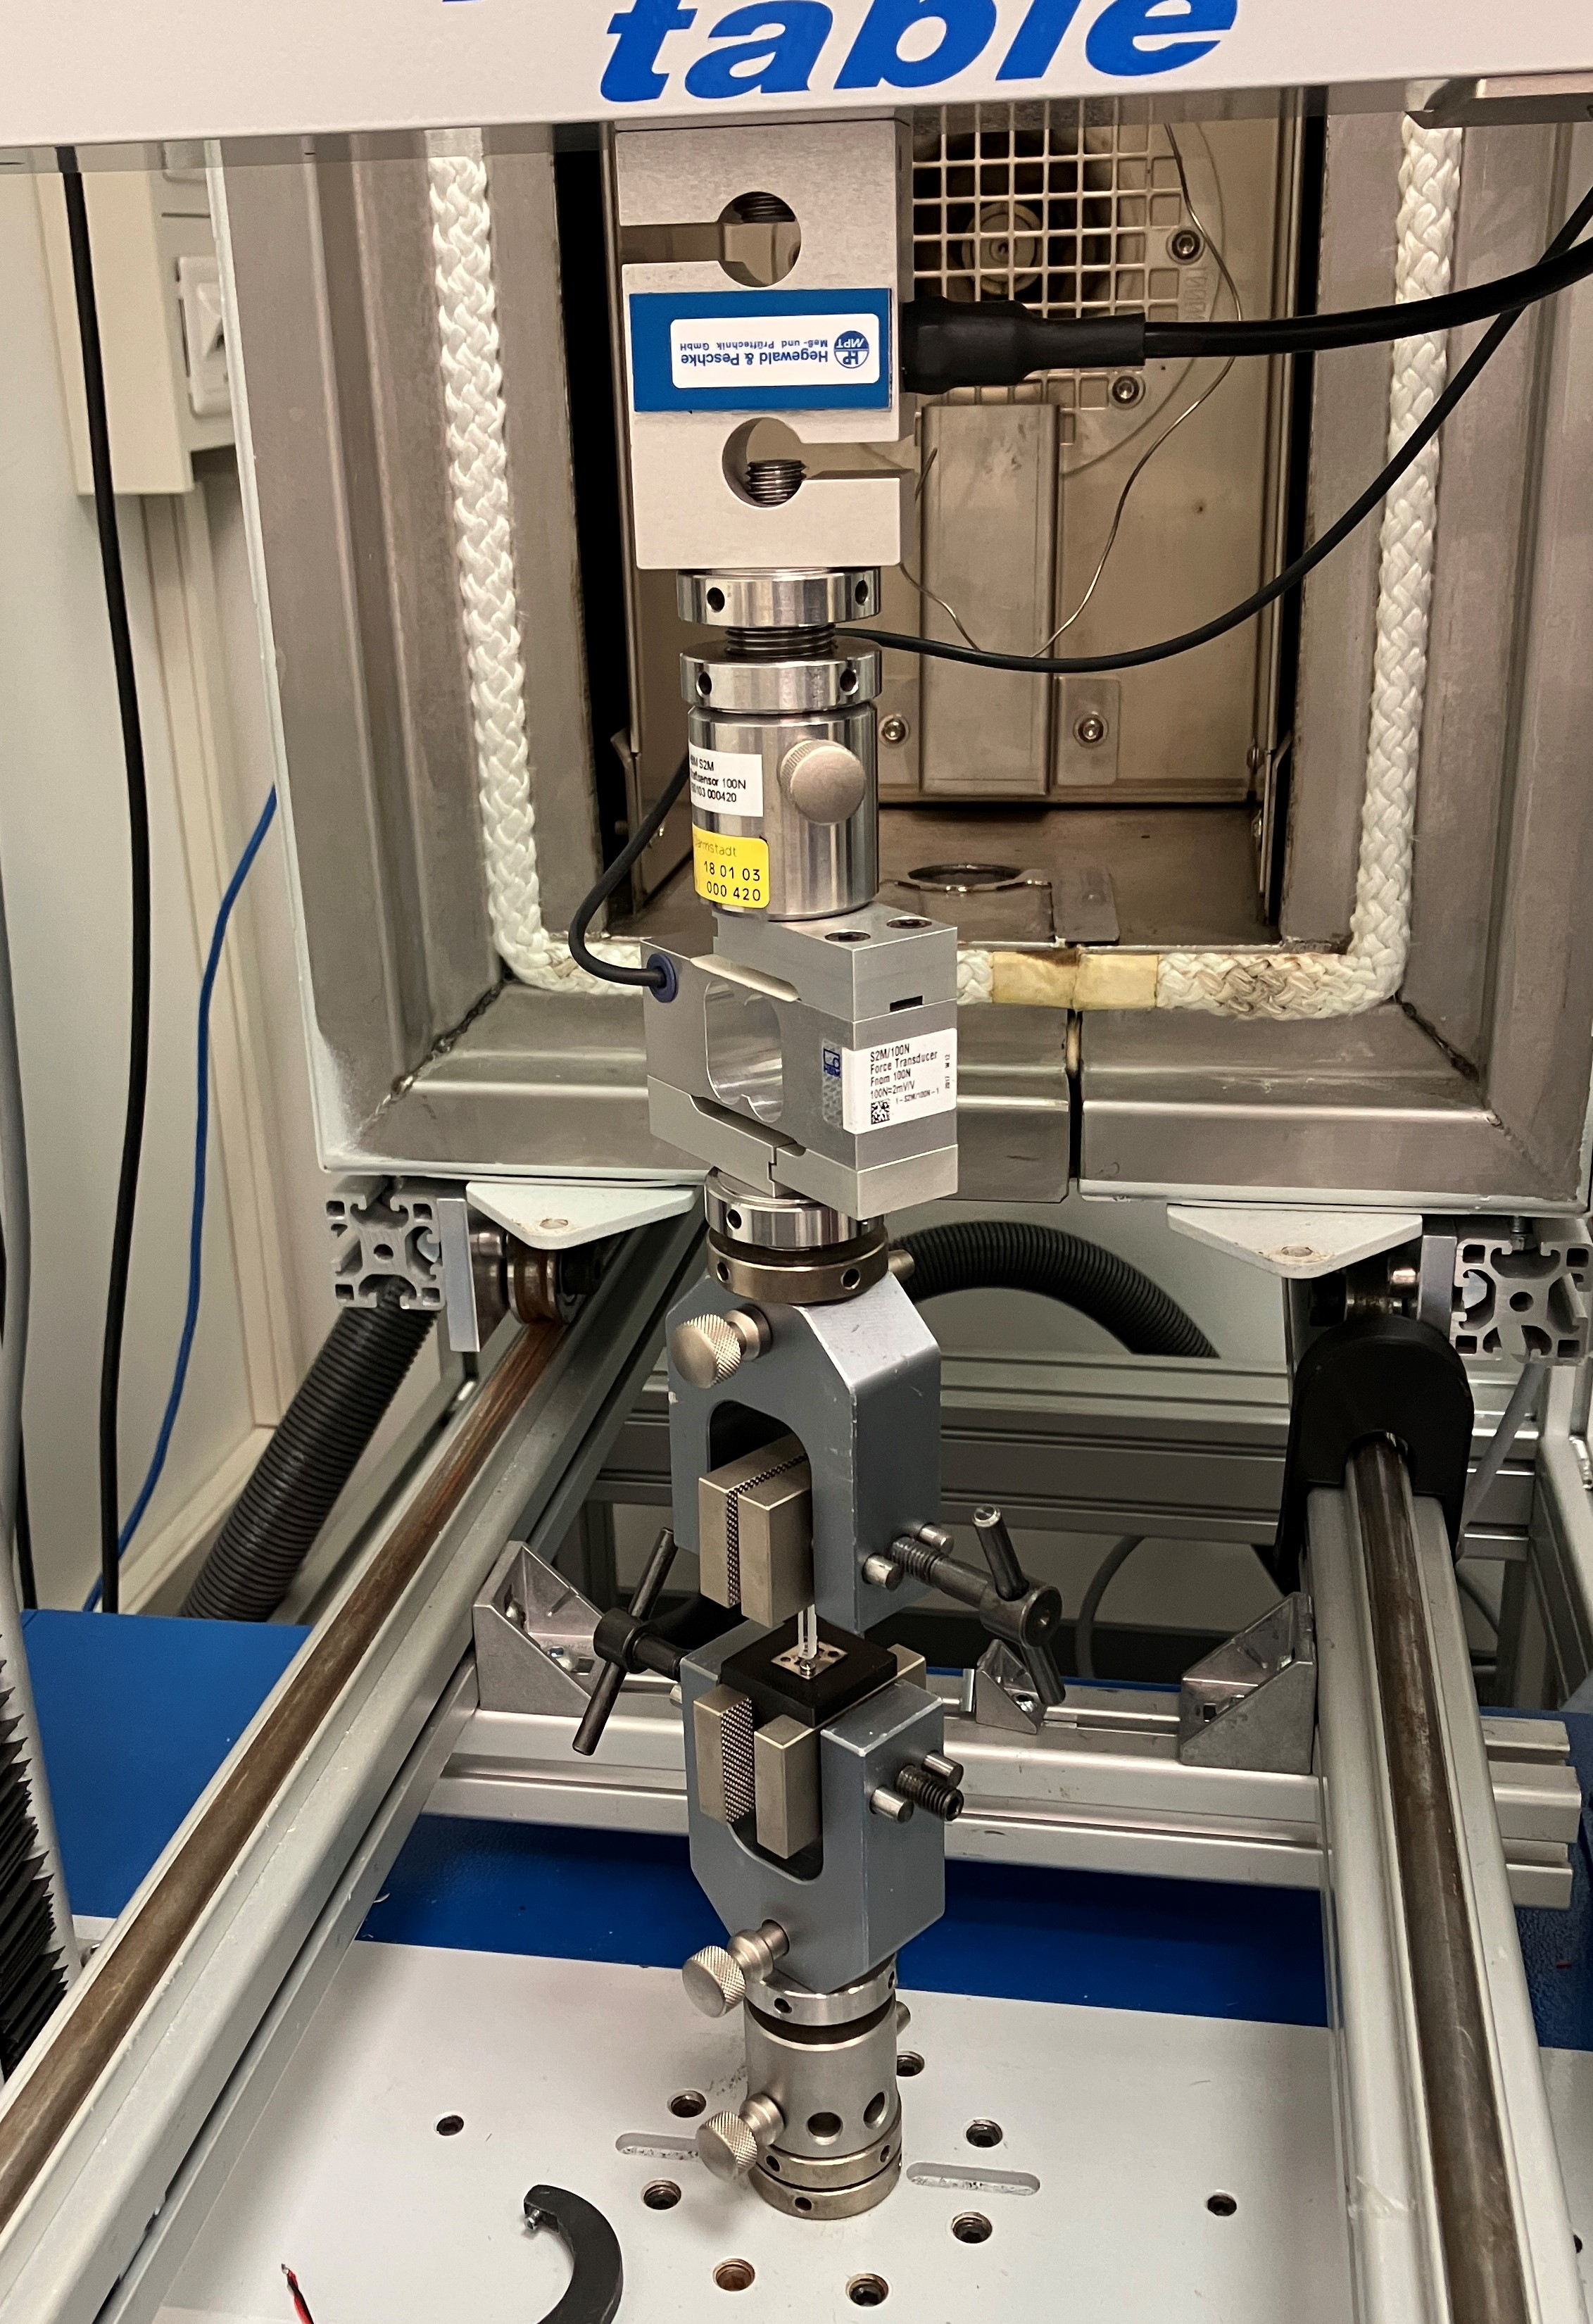
\includegraphics[width=6cm, height=9cm]{AufbauPullingMachine}
		\caption{}
	\end{subfigure}
	\begin{subfigure}[]{0.45\textwidth}
		\centering
		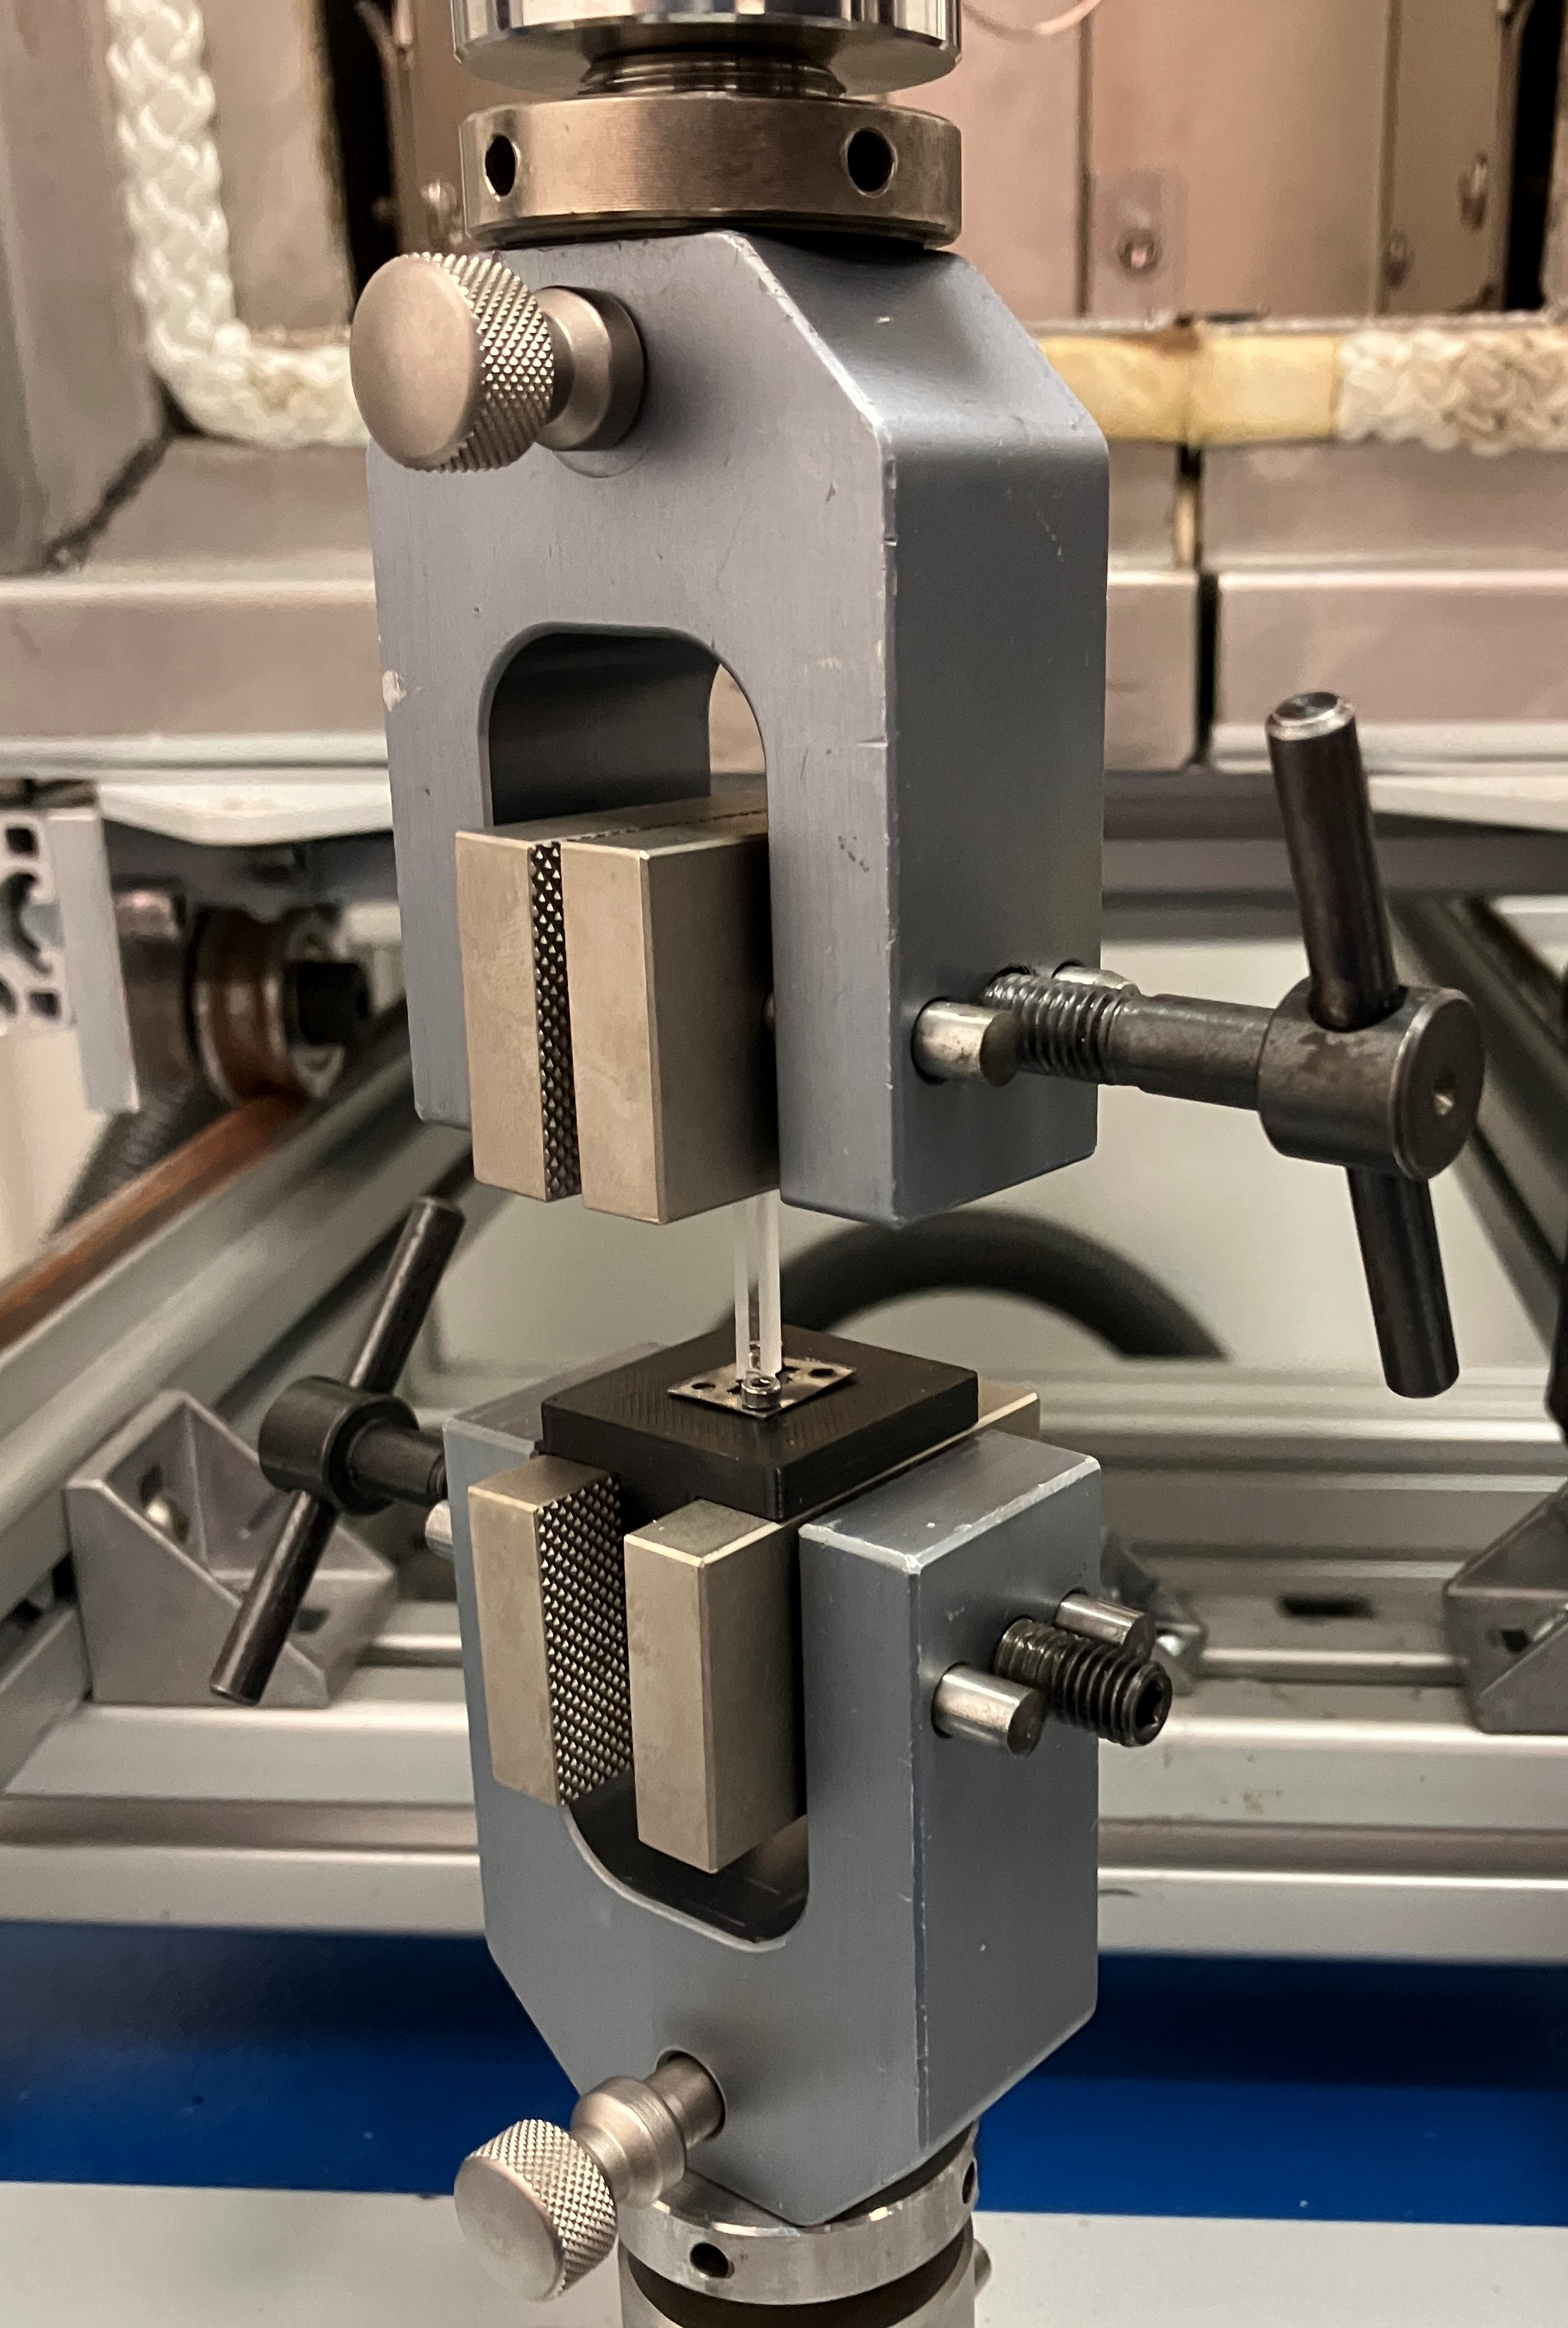
\includegraphics[width=6cm, height=9cm]{AufbauPullingMachineCloseup}
		\caption{}
	\end{subfigure}
	\caption{Setup on the Pulling Machine.}
	\label{fig:PullingMachineSetup}
\end{figure}

Because Glue dosaging varied a good amount, the Area is not assumed to be the bottom of the stamp. After Pulling, the glue is sticking on the stamp, outlining the area of the glue. The glue is analyzed under a microscope and the area is measured. With the Area and the maximum Force shortly before detaching, the Tensile stress is calculated. Then the experiment is repeated.



\subsection{detaching ice from PDMS}

1:2 and 4:1


	
\chapter{Results}

	% !TeX spellcheck = en_US


\section{Lipids}

In the previous chapter, the method of using a sacrificial layer to detach Ice was discussed. For this, lipids need to be solved at cryogenic temperatures. As not every lipid is solvable the same way in different solvents, a first test is conducted to obtain the potential solvents at room temperature. then the best solvents are also tested at cryogenic temperatures.

The solubility of lipids at room temperature in different solvents are tested. For this experiment the cover glasses are coated with lipids. Then a first reference image was taken. Then the cover glass is given into a small container with the potential solvent. After 15 minutes, the cover glass is removed and compared under the microscope with the reference picture. If streaks created from lipids are still as visible as before, the lipids are categorized as insoluble in this solvent. If the streaks partially dissapeared and/or are less visible, the lipids are categorized as partially soluble in this solvent. Last if the streaks completely disappear, the lipids are assinged as soluble in the solvent (Table \ref{table:LoeslichkeitRaumtemperatur}).


\begin{table}[hbt!]
	\centering
	\begin{tabular}{|l|c|c|}
		\hline
		potential solvent & solubility EGG-PC & solubility DOPC \\
		\hline
		\hline
		4-Methyl Pentene & soluble & N/A  \\ 
		\hline
		3-Methyl Pentene & slightly soluble & insoluble \\
		\hline
		1-Pentene & insoluble & insoluble \\
		\hline
		Isopentane & soluble & slightly soluble\\
		\hline
		1-Propanol & soluble & soluble\\
		\hline
		Pentane & soluble & insoluble\\
		\hline
		Ethanol & N/A & soluble\\
		\hline
	\end{tabular}
	\caption{result of solubility tests at room temperature. soluble indicates solvents which are able to visibly solve all lipids off a cover glass. slightly soluble indicates solutions which are able to solve lipids, but some stains are left: insoluble indicates no visible changes of tested lipid.}
	\label{table:LoeslichkeitRaumtemperatur}
\end{table}

This experiment shows that three different solvent exist for each EGG-PC as well as DOPC with high solubility (Table \ref{table:LoeslichkeitRaumtemperatur}). Following those results, solvents categorized with "soluble" are tested regarding solubility at temperatures of \SI{-140}{\degreeCelsius}. As not all solutions are liquid at \SI{-140}{\degreeCelsius} (Table \ref{table:SchmelztemperaturLösungsmittel}), they are tested at higher temperatures above their melting point, as mentioned in chapter \ref{chapter:meltingtemp}. In addition they are tested as mixtures with other solvents with a lower melting point, to lower its melting point. Additionally all lipids are tested in liquid ethane. Ethane was not tested at room temperature, as the boiling point is at \SI{-88.6}{\degreeCelsius} (ZITAT PUBCHEM ETHANE).

This experiment shows that no tested solvent was able to completely solve lipids at \SI{-140}{\degreeCelsius} and within \SI{15}{\minute} (Table \ref{table:Cryoloeslichkeit}). Also the smears of lipids did not only stay partially behind, but also new streaks appear on the glass slides. This means that some lipids redistributed on the glass slide.

Using solvents to destroy a sacrificial layer, a high solubility is a requirement. In this case, the sacrificial layer would be completely covered by the ice layer except the edges. So the solvents have only a small area to start solving the layer. To solve it completely, a strong solvent is needed to detach the ice layer from the slide. Additionally, as the ice layer needs to stay vitrified, the temperature cannot be raised over \SI{-140}{\degreeCelsius}. 

The solving process of lipids in solutions is probably endothermic. This means that heat is needed to solve lipids, so cold temperature heavily decrease solubility QUELLE DENNIS ODER SO. This effect was observed over the last experiments by all solvents to varying degree. It can be assumed that the majority of solvent lipids mixtures are endothermic which is very disadvantageous for finding a potential solvent lipid candidate. Strongly exothermic solvents could heat up the ice enough to create ice crystals, which would not be feasible. So only weakly exothermic solvents are feasible for this task. 

\begin{table}[hbt!]
	\begin{subtable}{\linewidth}
		\centering
		\begin{tabular}{|l|l|}
		\hline
		Solvent & Result \\
		\hline
		\hline
		Pentane & soluble at \SI{-125}{\degreeCelsius} \\
		\hline
		4-methyl pentene & insoluble \\
		\hline
		\makecell[l]{1:1 volume ratio\\ HFE to 1-Propanol} & \makecell[l]{did not mix,\\ slightly soluble}\\
		\hline
		Liquid ethane & insoluble\\
		\hline
		\end{tabular}
		\caption{EGG-PC}
		\label{table:EGG-PCCryoloeslichkeit}
	\end{subtable}
	\begin{subtable}{\linewidth}
		\centering
		\begin{tabular}{|l|l|}
		\hline
		Solvent & Result \\
		\hline
		\hline
		\makecell[l]{1:4 volume ratio\\ 1:2 molar ratio\\ Ethanol to Isopentane} & slightly soluble\\
		\hline
		\makecell[l]{1:2 volume ratio\\ 1:1 molar ratio\\ 1-Propanol to Isopentane} & insoluble \\
		\hline
		Isopentane & slightly soluble\\
		\hline
		1-Propanol & \makecell[l]{at \SI{-130}{\degreeCelsius}\\ slightly soluble}\\
		\hline
		Liquid ethane & insoluble \\
		\hline
		\end{tabular}
		\caption{DOPC}
		\label{table:DOPCCryoloeslichkeit}
	\end{subtable}
	\caption{ in \ref{table:EGG-PCCryoloeslichkeit} for EGG-PC, no sufficient solubility at -140°C was found. In \ref{table:EGG-PCCryoloeslichkeit}, DOPC was tested but also no proper solution was found.}
	\label{table:Cryoloeslichkeit}
\end{table}

As finding a good solvent lipid combinations seems very unlikely, a new method was tested. In the next section, the finger tool is used to try mechanically detach the ice layer.

\FloatBarrier
\section{Finger}

For this section, cover glass coated in Parylene are used as object slide. The slide is then dipped in solution containing lipids for a lipid coating. A ice layer with fluoriscine is frozen with either plunge-freezing or using a pincer and liquid nitrogen. Additionally, the "finger" is used as tool to try lifting off a piece of ice from the frozen layer on top of the lipids. In the next sections, different variables are examined and tested.

\subsection{Finding right dosage of HFE}

First obvious variable and potential issue source is the amount of HFE used as glue. High dosages of liquid hfe can spread underneath the frame holding the sample, leading to an inefficient force distribution. Also a big glue layer is a weak point between finger and sample, leading to a reduction of maximum force which can be applied. Too little glue will not connect the finger to the sample. Additionally, the dosaging of glue revealed to be a big challenge.

The HFE is dosaged with a pipette. The HFE is "taken up WORD" at room temperature, then the HFE is "released WORD" on the tip of the finger. In between, HFE is evaporating. Around $4\,\mu l$ is evaporating each time. Based on this knowledge, dosaging $4.10\,\mu l$, $4.30\,\mu l$ and $4.50\,\mu l$ is compared and a picture is made.

Results show that pipetting HFE is not reliable. The range spreads of too little to too much HFE even for those dosages. Not only differences in evaporation are playing a role. Correct placement on the tip is a major factor of glue dosaging. Still, a visual estimate for the correct glue dosage can be made by calculating the drop volume out of camera images.

\begin{figure}[hbt!]
	\centering
	\begin{subfigure}[]{0.45\textwidth}
		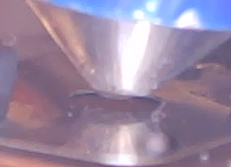
\includegraphics[width=6cm]{Temp_Picture_Lower_Limit}
		\caption{chosen example for lower limit}
	\end{subfigure}
	\begin{subfigure}[]{0.45\textwidth}
		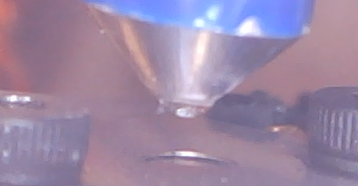
\includegraphics[width=6cm]{Temp_Picture_Upper_Limit}
		\caption{chosen example upper limit}
	\end{subfigure}
	\caption{example of upper limit and lower limit for glue dosages. (BETTER PICTURES NEEDED)}
\end{figure}

To calculate the actual glue dosage, two exemplary Pictures of an Upper and lower limit of glue dosages is picked. Then the Volume is calculated with a formula for the volume of a spherical section. All needed components are calculated out of the estimated contact angle of the glue $\alpha \approx 45°$ and the tip diameter of $d = 1.68\,mm$, for the lower range a reduction of $d$ by a factor of $\frac{2}{3}$ is assumed as the drop is not covering the whole tip. The resulting volume range of the glue dosage is $ 0.11\,\mu l \gtrapprox V \gtrapprox 0.38\,\mu l $. Also the lower end of this range is desired, but the repetition range in correctly dosaging lower doses is lower.

\subsection{Temperature over applied force}

As the HFE gluing effect is temperature dependent, the temperature needs to be regulated precisely. To narrow in the temperature dependency of HFE, the properties of HFE are observed at different temperatures in a regulated bath. Between -160°C and -170°C, the HFE is increasingly viscious. Under this temperature, HFE Freezes and gets brittle. Over this temperature range, HFE is too fluid to transfer any tensile forces. 

In application tests on lipid samples, the temperatures -160°C, -165°C and -170°C are compared. It was observed that decreasing temperatures lead to higher forces transferred to the sample. At the same time, temperatures are not reliably reached under -160°C.
As lower temperatures leads to an additional factor for repeatability issues, -160°C is used all other experiments.

\subsection{Tensile mode vs Shear mode}



\subsection{Detaching ice with finger of plunge freezed samples}

Next observed possible factor is the thickness of the ice layer. In the following, samples freezed with a plunge-freezer are compared to samples freezed with a pincer in liquid nitrogen. The results are categorized in 4 categories: Not successful pulls don't have visible changes of the flourescent ice layer, Partially successes are visible breaks or clear movement of ice parts on the ice layer, Successful liftoff is a missing piece and a visible piece on the finger, which could be used for future steps. In the results, there is no difference between Hand freezed and plunge-freezed samples regarding detachability. Therefore Ice thickness is not a factor which makes detaching ice easier. As both methods don't show success in detaching ice pieces, it could still be a relevant factor but not a thing which should make a certain solution magically work xD

\subsection{other observed error sources??}

Wrong positioning, forming of ice

\begin{table}
	\centering
	\begin{tabular}{|c|c|c|}
		\hline
		Category & Hand-freezed & Plunge-freezed \\
		\hline
		\hline
		count executed tries & 4 & 4\\
		\hline
		unsuccessful & 3 & 3\\
		\hline
		breaks/movement of ice & 1 & 1\\
		\hline
		piece lifted with finger & 0 & 0\\
		\hline		
	\end{tabular}
	\caption{Comparison of detachability between hand-freezed and plunge-freezed samples}
\end{table}

\section{PDMS}

Now two mixture ratios of PDMS are compared. For this, samples where coated with 4:1 and 1:2 curing agent to base coat weight ratio. Also for ..., glass without pdms is used. The pulling mashine was used to determine the max force. A plexiglass stamp was used for pulling off the PDMS layer. UV Glue was used to fixate the plexiglass onto the PDMS and is cured with 3 min UV exposure. After pulling, the Area of the separating layers is determined via microscope. Then the max pulling tension is calculated. This was repeated several times. The Result shows, that glass is hardest do pull off. Then 4:1 is harder to separate than 1:2 (Fig. \ref{fig:vgl4:1zu1:2zuGlas}). In literature, 1:2 weight ratio should have a lower adhesion force on ice too\cite{IbanezIbanez.2022}. For those reasons, 1:2 was picked to continue experiments with plasma treatment.

\begin{figure}
	\centering
	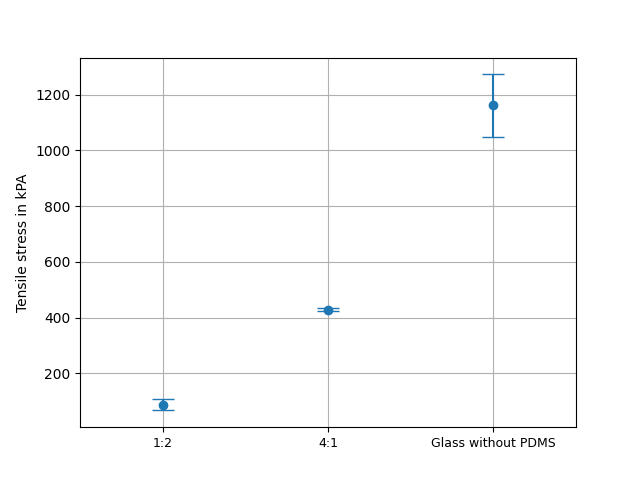
\includegraphics[width=14cm]{plotVGLZugspannungPDMSMischungsverhaeltnisse}
	\caption{Comparison 4:1, 1:2 Base coat to curing Agent and glass without PDMS}
	\label{fig:vgl4:1zu1:2zuGlas}
\end{figure}

\begin{figure}
	\centering
	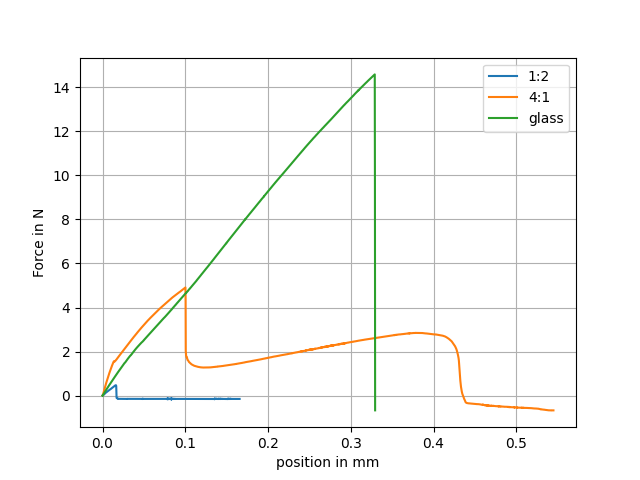
\includegraphics[width=14cm]{ForceOverTime}
	\caption{force over Time}
\end{figure}

In the next experiment, the effect of plasma curing is investigated. The same setup is used. Samples with a 2:1 weight ratio are additionally plasma treated before quickly clamping on the pulling mashine. Even with low repetition rates, a clear tendency can be observed. With lower and stronger plasma treatment, the durable the PDMS Layer gets (Fig. \ref{fig:PlotPlasmaAktivierung}). Over the whole range, The needed stress sextubles. Because the repititon rate is low, the exact values should be treated cautiosly. Also the results are not applicable to other mixture ratios, as different behaviour in plasma activation was observed between 2:1 and 4:1 weight ratio. also no glass-like state was observed in 2:1 weight ratio mixture.


\begin{figure}[h]
	\centering
	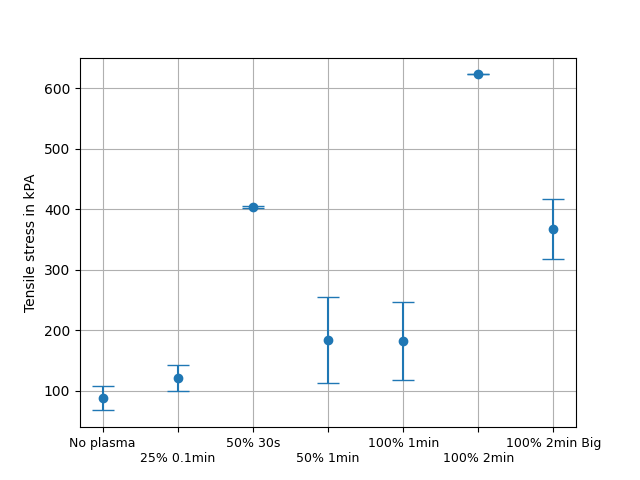
\includegraphics[width=14cm]{plot2_1PlasmaAktivierung}
	\caption{PDMS 2:1 Comparison between various Plasma curing strengths and durations.}
	\label{fig:PlotPlasmaAktivierung}
\end{figure}




	
%\chapter{Discussion (VIELLEICHT IN ERGEBNISSE)}

	%es gibt nichts zu diskutieren. 
	
\chapter{Conclusion}

	% !TeX spellcheck = en_US

%TODO Kurzfassung schreiben.
In conclusion, tested methods are not sufficient to separate the ice layer from a sample holder. Solvent used for lipids are generally endothermic. Some solubility is reached at cryogenic temperature, but not enough to completely dissolve a lipid layer. A successful separation was made with 4:1 mixture ratio PDMS, but the reproducibility must be shown in future work.

PDMS is tuned at room temperature. Results have confirmed a connection between adhesion forces measured in papers and at tensile testing. Plasma activation has the opposite effect of 1:2 mixture ratio than on 50:1 mixture ratio. The surface gets more stable with increasing plasma activation instead of more brittle.

The finger with HFE is able to apply tensile stress between \SI{103.3}{\kilo\pascal} and \SI{585.4}{\kilo\pascal}. The stress applied is a couple magnitude higher than the stress calculated for detaching PDMS. The discrepancy could be result of energy lost deforming HFE at cryogenic temperatures and the stability of a continuous ice layer.

Different factors which increase and decrease the effectiveness of the finger: Too much HFE results in HFE ripping because of the low cohesion. Too little HFE is prone to not properly attaching to the Sample. lower temperature increase the viscosity and therefore stability of HFE. But at around \SI{-170}{\degreeCelsius}, cracks form in HFE and the strength is drastically reduced.

The direction of force could help at detaching an ice layer. However, the observed stability to shear load of HFE is considerably lower than to tensile load. The ice structure is not negletable. A continuous ice layer has more adhesion to the sample than an already broken layer. 

Positioning is also important, expecially keeping the correct gap between sample and finger in which the HFE is spread thin but not flows between window and sample. Also slow temperature changes are drastically reducing the likelyhood of a good connection between sample and finger.

At room temperature, the PDMS with different mixture ratios were tested. A mixture ratio of 1:2 has shown low adhesion forces as predicted. However, the transfer of results at room temperature to ice adhesion at cryogenic temperatures is only possible with restrictions. Plasma activation increases the adhesion forces potentially more on ice than the UV glue. At other mixture ratios, plasma treatment leads to brittle surfaces, which is not observed for 1:2 mixture ratio. Attempts of detaching an ice layer off this PDMS coated sample were not successful.

Additionally, A PDMS mixture of 4:1 and 1:50 were investigated. With plasma treatment with $100\,\%$ power and \SI{10}{\minute}, Cracks form and the surface is brittle. However, The ice layer frozen on top of a PDMS coated sample is continuous. Ions produced in plasma treatment increase the adhesion force too much for the finger to detach. In future, stress needed to break the ice layer should be taken into account. Also to decrease the area of contact to the slide, a grid could be used to reverse the hydrophilic effect of plasma activation before freezing. The resulting small pieces of ice may be easier to detach than a clamped down continuous layer.

In contrast to PDMS coated slides, lipid coated slides resulted in cracks in the ice layer itself. In pulling tests with the finger, breaking and moving parts of the ice layer were possible in 1 out of 4 cases. To help detach the lipid layer, PDMS could be used. With increased brittleness and pre broken ice layer, less stress is needed for detaching.

In Experiments, no lipid solvent combination was found with high solubility at cryogenic temperatures. All tested solving processes are endothermic. In general, endothermic processes are inefficient in cold temperatures.

The potential for lipids and detergents is not exhausted in this thesis. lipids and detergents can be engineered for lower adhesion forces. Additionally, finding solvents by solely experiments is very unlikely. 

To engineer a sacrificial layer, other detergents could be used \cite{SigmaAldrich.2023}. An exothermic process is also not limited through the cyrogenic temperatures. Alternatively, to increase solubility, changing the pH value of lipid and solvent could increase solubility \cite{BruceA.AverillPatriciaEldredge.}.

The force applied of the "finger" has proven to be not enough to break any surface on the sample. Pre broken pieces are sometimes picked up. A process is needed to completely loosen the ice layer without the "finger". For example, deactivating the plasma by putting a grid on the PDMS after Plasma activation could result in a loose, incontinuous but regular layer. Smaller pieces with less adhesion are easier to detach.

In general, the finger setup is not reliable. Even after analysis, forces applied with the finger vary too much for inducing strong forces to a sample. However, pre broken pieces may be able to be picked up easier. Therefore, other methods of breaking loose the ice layer should be searched.

Another way to create a loose ice layer is to engineer the ice layer itself. Additives inside the ice layer could help in the breaking process. Freezing the ice in an emulsion could result in an incontinuous ice layer. 



\chapter{References}
\printbibliography[heading=none]

\end{document}
